\chapter{Metodologi dan Rancangan}

\section{Alur Pengembangan}

Pengembangan sistem yang akan dibangun mengikuti alur yang terdapat pada Gambar \ref{fig:waterfall}. Alur yang digunakan adalah alur \textit{waterfall}. Alur tersebut memungkinkan untuk kembali ke tahap sebelumnya jika pada tahap tertentu terjadi kesalahan. Tahap pertama dalam alur adalah penelitian. Penelitian dilakukan untuk menentukan algoritma yang cocok untuk diterapkan ke dalam sistem. Lalu, tahap kedua adalah perancangan sistem. Perancangan dilakukan untuk menentukan tahap-tahap yang akan dilakukan oleh sistem. Kemudian, tahap selanjutnya adalah pengembangan sistem, yang mana merupakan tahap untuk pengembangan dari rancangan sistem yang telah dibuat sebelumnya. Tahap terakhir pada alur pengembangan adalah pengujian sistem.

\begin{figure}[H]
	\centering
	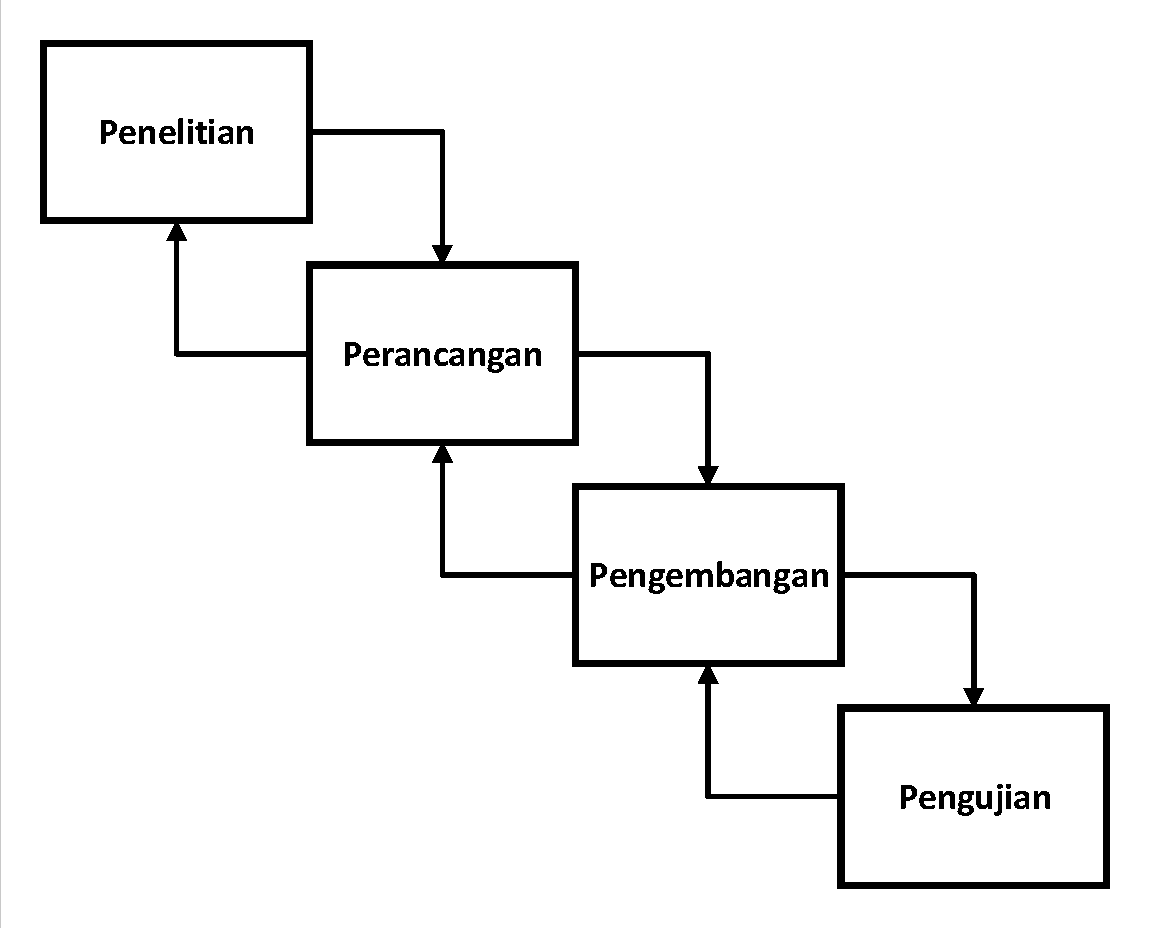
\includegraphics[width=0.7\textwidth, trim=2 2 2 2, clip]{resources/3/waterfall.pdf}
	\caption{Alur \textit{waterfall} untuk pengembangan sistem}
	\label{fig:waterfall}
\end{figure}

\section{Rancangan Latihan Klasifikasi}

Rancangan sistem untuk tahap latihan klasifikasi disajikan dalam bagan pada Gambar \ref{fig:design_training} berikut. Proses-proses yang harus dilewati dalam tahap latihan klasifikasi dapat dijelaskan sebagai berikut:

\begin{enumerate}
	\item sistem akan memuat \textit{file} JSON yang berisi data latihan yang digunakan untuk membangun NLU,
	\item sistem mengambil data latihan tersebut lalu mengubahnya menjadi sekumpulan obyek SentenceData,
	\item sistem mengambil informasi maksud kalimat yang telah didefinisikan di dalam data latihan dan menyimpan sekumpulan maksud kalimat,
	\item sistem memecahkan sebuah kalimat menjadi sekumpulan \textit{token} kata,
	\item sistem mengekstraksi entitas yang telah didefinisikan di dalam data latihan dan mengumpulkan semua entitas yang terekstrasi,
	\item sistem menciptakan tas kata-kata dengan menggunakan metode \textit{one-hot encoding},
	\item sekumpulan maksud kalimat dan tas kata-kata digunakan sebagai masukan untuk latihan model NLU, menghasilkan model klasifikasi, dan,
	\item model klasifikasi disimpan ke dalam direktori sistem untuk digunakan pada tahap klasifikasi teks.
\end{enumerate}

\begin{figure}[H]
	\centering
	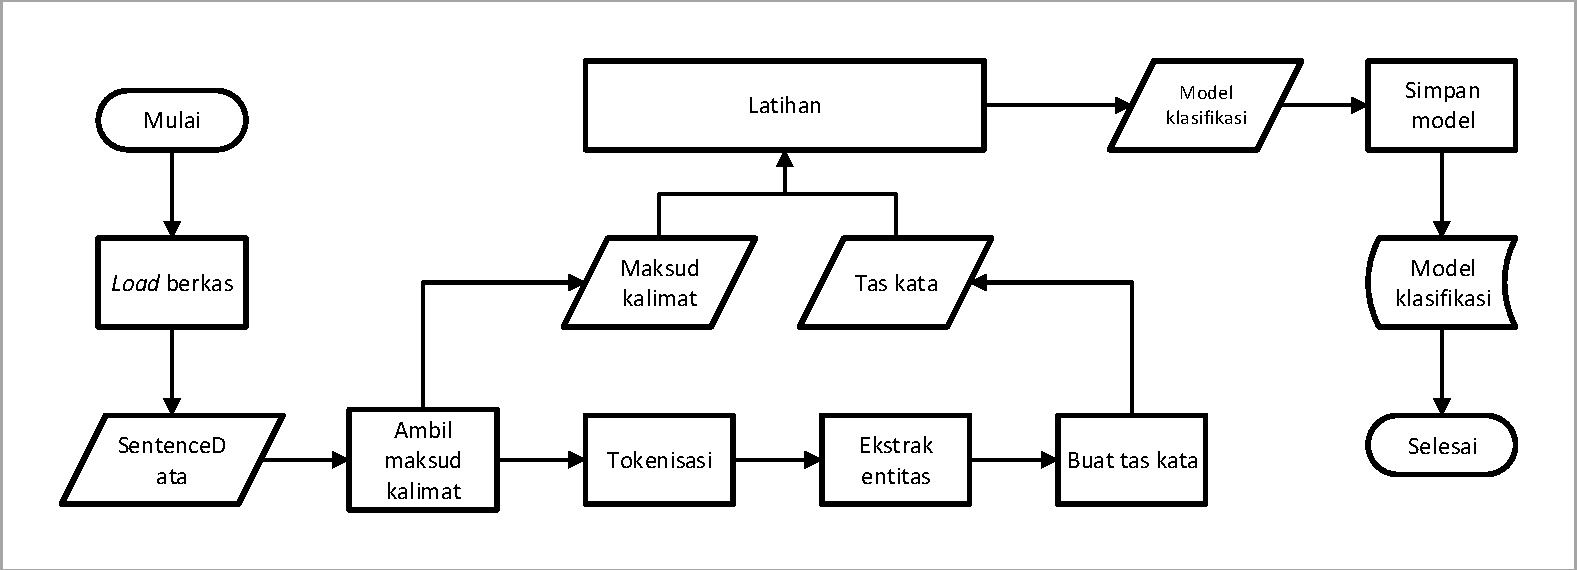
\includegraphics[width=\textwidth, trim=2 2 2 2, clip]{resources/3/design_training.pdf}
	\caption{Bagan rancangan sistem tahap latihan klasifikasi}
	\label{fig:design_training}
\end{figure}

\section{Rancangan Klasifikasi Teks}

Rancangan sistem untuk tahap klasifikasi teks disajikan dalam bagan pada Gambar \ref{fig:design_classification}. Proses-proses yang harus dilewati dalam tahap klasifikasi teks dapat dijelaskan sebagai berikut:

\begin{enumerate}
	\item sistem menerima masukan teks dari \textit{speech recognition} yang dimasukkan oleh suara pengguna,
	\item sistem memecahkan teks menjadi sekumpulan \textit{token},
	\item sistem mengenali entitas yang berada di dalam teks, kemudian mengekstraksi entitas tersebut,
	\item sistem menciptakan tas kata-kata untuk teks masukan,
	\item sistem melakukan prediksi maksud kalimat dari masukan tas kata-kata menggunakan model klasifikasi yang dihasilkan pada tahap latihan klasifikasi,
	\item maksud kalimat yang telah dihasilkan, bersama dengan kumpulan entitas hasil ekstrasi, menjadi masukan untuk memenggil aksi sistem, dan,
	\item sistem melakukan aksi kepada pengguna sebagai tanggapan dari masukan teks dari sistem ASR.
\end{enumerate}

\begin{figure}[H]
	\centering
	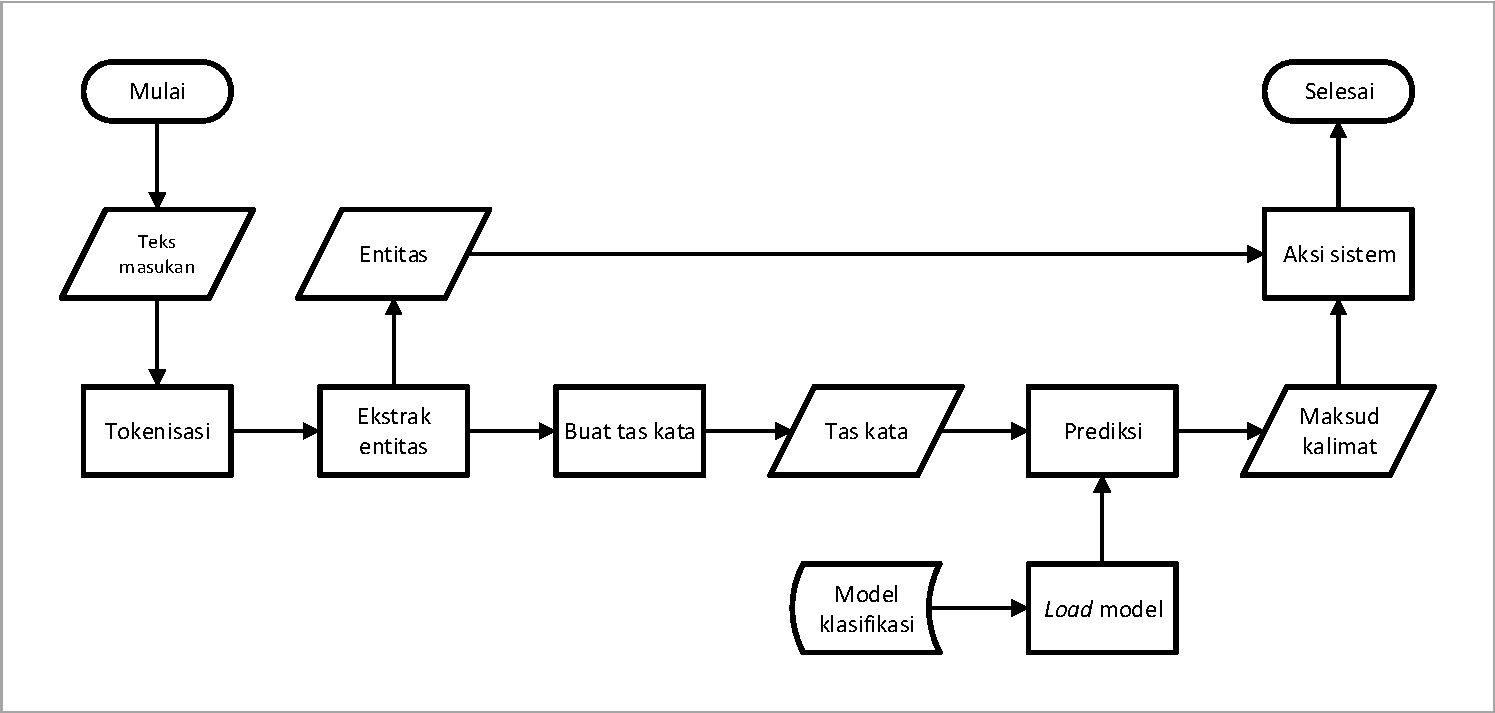
\includegraphics[width=\textwidth, trim=2 2 2 2, clip]{resources/3/design_classification.pdf}
	\caption{Bagan rancangan sistem tahap klasifikasi teks}
	\label{fig:design_classification}
\end{figure}

\section{Algoritma untuk Pelatihan Pengenalan Entitas}

Teknik yang dilakukan untuk bagian pengenalan entitas adalah teknik \textit{sequence labeling}, seperti yang tertera pada Gambar \ref{fig:sequence_labelling}. Sebuah kalimat yang disediakan oleh data latih menyertakan kata-kata yang merupakan bagian dari entitas. Kalimat tersebut dipecahkan menjadi \textit{token-token}. Tiap \textit{token} berisi sebuah kata dalam kalimat. Tiap \textit{token} ditandai dengan label-label, menandakan apakah \textit{token} tersebut merupakan entitas atau tidak. Susunan \textit{token} dan label tersebut akan menjadi acuan untuk pelatihan pengenalan entitas.

\begin{figure}[H]
	\centering
	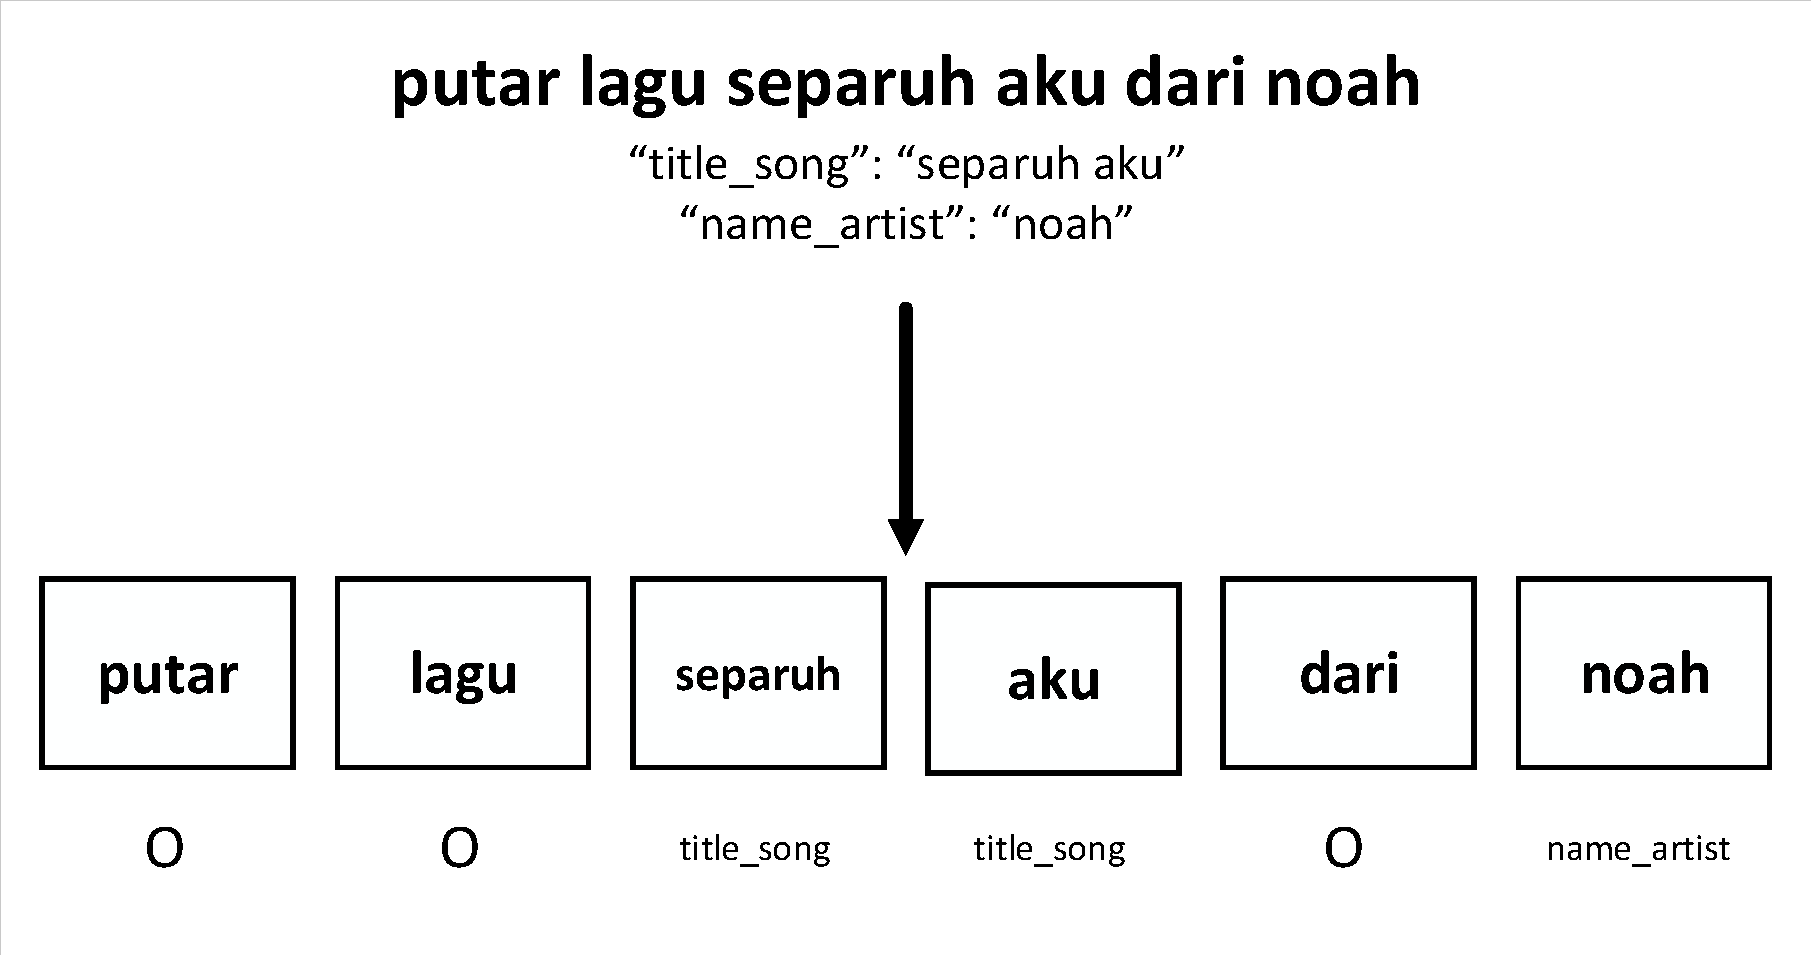
\includegraphics[width=0.9\textwidth, trim=2 2 2 2, clip]{resources/3/sequence_labelling.pdf}
	\caption{Teknik \textit{sequence labelling}}
	\label{fig:sequence_labelling}
\end{figure}

Melihat kelemahan yang terdapat pada pengenalan entitas milik Rasa NLU, beberapa variasi algoritma dapat digunakan untuk mengganti pelatihan pengenalan entitas tersebut.

\subsection{\textit{Convolutional Neural Network} (CNN)}

\textit{Convolutional neural network} atau CNN biasa digunakan untuk mengenali objek-objek yang berada di dalam sebuah gambar. CNN mencoba memprediksi sebuah objek yang bersangkutan dengan mendeteksi fitur-fitur yang terdapat dalam sebuah gambar menggunakan \textit{filter}. Untuk penerapan di dalam teks, fitur-fitur tersebut didapatkan dengan melakukan \textit{embedding} pada sebuah kata yang bersangkutan. \textit{Embedding} adalah proses untuk merepresentasikan sebuah kata menjadi vektor multi dimensi.

Keuntungan yang dimiliki oleh CNN, jika dibandingkan dengan \textit{recurrent neural network} (RNN), adalah kemampuan CNN dalam melihat kata yang berada di depan satu kata yang sedang dilatih. Dengan begitu, CNN dapat mempertimbangkan kata sebelum dan kata selanjutnya untuk memasangkan label pada sebuah kata.

Gambar \ref{} menunjukkan arsitektur lapisan CNN yang digunakan untuk melakukan latihan pengenalan entitas ini, dibangun dengna menggunakan Keras. Lapisan pertama diawali dengan melakukan \textit{embedding} terhadap kumpulan kata dalam sebuah kalimat yang ingin dilatih. Kemudian, hasil \textit{embedding} dimasukkan ke lapisan \textit{convolutional} satu dimensi. Selanjutnya, luaran dari lapisan \textit{convolutional} dikurangi sebesar 0,25 persen pada lapisan \textit{dropout}. Hal ini bertujuan untuk meningkatkan kinerja pembelajaran sebuah model. Setelah itu, luaran yang telah dikurangi dimasukkan ke dalam lapisan \textit{gated recurrent unit} (GRU). Terakhir, luaran GRU dimasukkan ke lapisan \textit{neural network} yang terdistribusi berdasarkan \textit{timestep} dengan menggunakan pembungkus TimeDistributed.

\subsection{LSTM Dua Arah dan CRF}

\textit{Long short term memory} atau LSTM digunakan untuk mengatasi permasalahan latihan dengan menggunakan data yang bersifat \textit{sequential}. LSTM digunakan untuk mengatasi kelemahan yang dimiliki oleh RNN, yaitu RNN tidak mampu menyimpan informasi dalam jangka waktu yang sangat lama. LSTM dapat memutuskan apakah sebuah informasi akan diteruskan pada iterasi berikutnya atau dilupakan dengan bantuan dari gerbang pelupa (\textit{forget gate}).

Gambar \ref{} menunjukkan isi dari sebuah sel LSTM. Sel LSTM terdiri dari empat jenis gerbang, yaitu dua gerbang masukan, gerbang keluaran, dan gerbang pelupa. Semua gerbang mengandalkan masukan yang berasal dari masukan kata iterasi saat ini dan luaran dari iterasi sebelumnya. Kedua gerbang masuk mengolah nilai luaran dan masukan dengan menggunakan fungsi aktivasi sigmoid dan tanh, kemudian dilakukan operasi perkalian matriks pada kedua hasil tersebut. Gerbang pelupa mengolah kedua nilai dengan menggunakan fungsi aktivasi sigmoid. Terakhir, gerbang luaran mengolah kedua nilai dengan menggunakan fungsi aktivasi sigmoid.

Kemudian terdapat sebuah nilai yang disebut dengan nilai keadaan sel. Nilai keadaan sel saat ini didapatkan dengan mengalikan nilai keadaan sel sebelumnya dengan nilai luaran gerbang pelupa, lalu ditambahkan dengan hasil dari kedua gerbang masukan. 

\subsection{LSTM Dua Arah dan CNN}


